\documentclass{praktikum}
\usepackage{pgfplots}
\usepackage{amsmath}
\usepackage{amsfonts}
\usepackage{amssymb}
\usepackage{graphicx}
\usepackage{multirow}
\graphicspath{ {./} }

%====== Vyplňte údaje ======
%% dobrá rada na začátek - pokud nevíš, co měníš, zálohuj to, co funguje ;)

\jmeno{Matyáš Peroutík}
\kod{256371}
\rocnik{2023/2024}
\obor{AMT}
\skupina{}
\labskup{B}
\spolupracoval{Štěpán Pavlica}


\ucitel{}
\merenodne{28.\,2.\,2024}
\odevzdanodne{13.\,2.\,2024}

\priprava{}
\opravy{}
\nazev{Vlastnosti ručkových měřících přístrojů}
\cislo{17} %měřené úlohy



\begin{document}
%====== Vygenerování tabulky ======
\maketitle
\vspace{0.5 cm}

%====== Text protokolu zde ======

\section{Úkol měření}
\paragraph{}
Zobrazte na osciloskopu a změřte zadané hodnoty napětí s harmonickým průběhem, a to neusměrněné a jednocestně i dvoucestně usměrněné. Využijte podle možnosti všechny voltmetry u úlohy.
\section{Teoretický rozbor}

\subsection{Efektivní hodnota elektrických veličin}
\paragraph{}
Efektivní hodnota elektrické veličiny je hodnota stejnosměrné stálé veličiny, která by za dobu jedné periody signálu na stejném ideálním rezistoru vyzářila stejné teplo. Z této definice vyplývají následující vztahy:

\begin{equation}
\label{eqn:u_effective}
U_{ef}=\sqrt{\frac{1}{T}\int_{0}^{T}u^2(t)dt}\
\end{equation}
\begin{equation}
\label{eqn:i_effective}
I_{ef}=\sqrt{\frac{1}{T}\int_{0}^{T}i^2(t)dt}
\end{equation}

kde u(t) je okamžitá hodnota napětí a i(t) je okamžitá hodnota proudu.

\subsection{Střední hodnota elektrických veličin}
\paragraph{}
Efektivní hodnota elektrické veličiny je hodnota stejnosměrné stálé veličiny, která by za dobu jedné periody signálu umožnila přenos stejně velkého náboje. Taky se jí občasně říká stejnosměrná složka signálu. Z definice vyplývají následující vztahy:

\begin{equation}
\label{eqn:u_meanval}
U_{s}=\frac{1}{T}\int_{0}^{T}u^2(t)dt\\
\end{equation}
\begin{equation}
\label{eqn:i_meanval}
I_{s}=\frac{1}{T}\int_{0}^{T}i^2(t)dt\\
\end{equation}

kde u(t) je okamžitá hodnota napětí a i(t) je okamžitá hodnota proudu.

\subsection{Střídavé napětí}
\paragraph{}
Tímto termínem se většinou myslí střídavé napětí harmonického sinusového průběhu. V laboratořích se používá zmenšené napětí síťě, které je transformováno v přípravku s transformátorem. Průběh tohoto napětí je popsán vzorcem:

\begin{equation}
\label{eqn:ut_stridave_harmonicke}
u(t)=U_M\cdot\sin(\omega t)=U_M \cdot \sin(2 \pi ft)
\end{equation}

kde u(t) je okamžitá hodnota napětí v čase t, $U_M$ je amplituda, $\omega$ je úhlová rychlost dána vztahem:

\begin{equation}
\label{eqn:omega_uhlova_rychlost}
\omega = 2 \pi f = \frac{2 \pi}{T}
\end{equation}

kde f je frekvence signálu a T je perioda signálu. Stejné vztahy platí pro proud.

\begin{center}
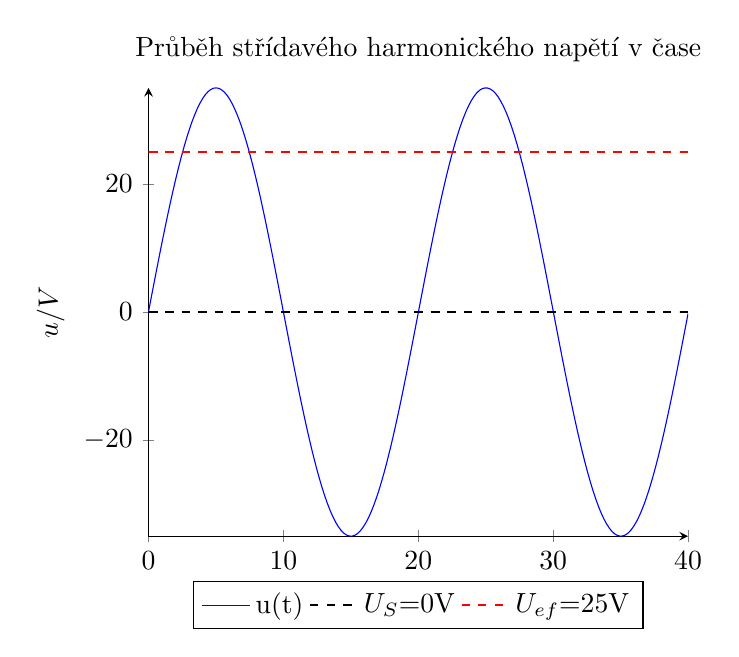
\begin{tikzpicture}
\label{grf:u_harmonic}
\begin{axis}[
    title = {Průběh střídavého harmonického napětí v čase},
    axis lines = left,
    xlabel = \(t/ms\),
    ylabel = {\(u/V\)},
    legend style={at={(0.5,-0.1)}, anchor=north,legend columns=-1},
]

%Sinusovka
\addplot [
	domain=0:40,
	samples=200,
	color=blue,
]
{35*sin(deg(2*3.14*50*x/1000))};
\addlegendentry{u(t)}

%mean 
\addplot [
	domain=0:40,
	samples=200,
	color=black,
	thick,
	dashed,
]
{0};
\addlegendentry{$U_S$=0V}

%effective 
\addplot [
	domain=0:40,
	samples=200,
	color=red,
	thick,
	dashed,
]
{25};
\addlegendentry{$U_{ef}$=25V}

\end{axis}
\end{tikzpicture}
\end{center}

\paragraph{}
Pro tento průběh je možno použít zjednoduššené verze vzorců (\ref{eqn:u_effective}) a (\ref{eqn:i_effective}). Jejich tvar poté bude následující:

\begin{equation}
\label{eqn:u_effective_harmonic}
U_{ef} = \frac{U_M}{\sqrt{2}}
\end{equation}

\begin{equation}
\label{eqn:i_effective_harmonic}
I_{ef} = \frac{I_M}{\sqrt{2}}
\end{equation}

Střední hodnoty proudů (\ref{eqn:i_meanval}) a napětí (\ref{eqn:u_meanval}) jsou u harmonického signálu rovny nule.

\subsection{Jednocestně usměrněné střídavé napětí}
\paragraph{}
Pokud pustíme výše definovaný signál střídavého harmonického napětí přes jednocestný usměrňovač (obvykle tvořen polovodičovou diodou) dostaneme nový signál, který nazýváme jednocestně usměrněné střídave napětí (proud). Tento průběh bude mít následující průběh:

\begin{center}
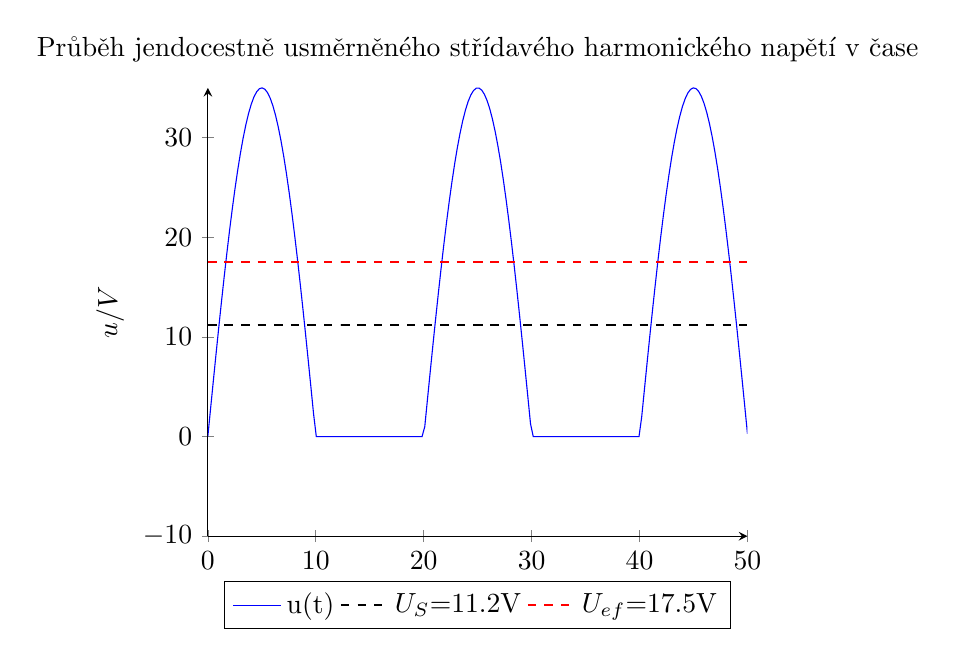
\begin{tikzpicture}
\label{grf:u_single_rectified}
\begin{axis}[
    title = {Průběh jendocestně usměrněného střídavého harmonického napětí v čase},
    axis lines = left,
    ymin = -10,
    xlabel = \(t/ms\),
    ylabel = {\(u/V\)},
    legend style={at={(0.5,-0.1)}, anchor=north,legend columns=-1},
]

%Sinusovka
\addplot [
	domain=0:50,
	samples=200,
	color=blue,
]
{35*sin(deg(2*3.14*50*x/1000))*((35*sin(deg(2*3.14*50*x/1000)))>0)};
\addlegendentry{u(t)}

%mean 
\addplot [
	domain=0:50,
	samples=200,
	color=black,
	thick,
	dashed,
]
{11.2};
\addlegendentry{$U_S$=11.2V}

%effective 
\addplot [
	domain=0:50,
	samples=200,
	color=red,
	thick,
	dashed,
]
{17.5};
\addlegendentry{$U_{ef}$=17.5V}

\end{axis}
\end{tikzpicture}
\end{center}

\paragraph{}
Po jednocestném usměrnění můžeme signál popsat následujícím vztahem

\begin{equation}
\label{eqn:ut_single_rect}
\begin{split}
u(t) = U_M \sin(2 \pi ft)  & \textsf{........pro }  \sin(2 \pi ft) > 0 \\
u(t) = 0 & \textsf{........pro } \sin(2 \pi ft) < 0
\end{split}
\end{equation}

\paragraph{}
Po dosazení průběhu (\ref{eqn:ut_single_rect}) do rovnic (\ref{eqn:u_effective}) (\ref{eqn:i_effective}) (\ref{eqn:u_meanval}) a (\ref{eqn:i_meanval}) dostaneme následující vztahy pro proudy a napětí tohoto signálu.

\begin{equation}
\label{eqn:u_eff_mean_single_rect}
U_{ef} = \frac{U_M}{2} \quad \quad \quad 
U_S = \frac{U_M}{\pi}
\end{equation}

\begin{equation}
\label{eqn:i_eff_mean_single_rect}
I_{ef} = \frac{I_M}{2} \quad \quad \quad 
I_S = \frac{I_M}{\pi}
\end{equation}

\subsection{Dvoucestně usměrněné střídavé napětí}
\paragraph{}
Pokud bychom na signál místo jednocestného usměrňovače, jak tomu bylo v minulé sekci, použili dvojcestný usměrňovač (obvykle realizován pomocí Gretzova oboucestného usměrňovače, resp. Gretzova můstku) dostaneme signál, který oproti jednocestně usměrněnému nemá nulovou hodnotu signálu po dobu půlky periody. Signál, který je na výstupu tohoto můstku je tedy absolutní hodnotou vstupního signálu, tudíž můžeme napsat následující vztah:

\begin{equation}
\label{eqn:ut_fullbridge_rect}
u(t) = U_M \cdot |\sin(2 \pi ft)|
\end{equation}

\paragraph{}
Tento signál bude mít podle vztahů (\ref{eqn:u_effective}) (\ref{eqn:i_effective}) (\ref{eqn:u_meanval}) a (\ref{eqn:i_meanval}) vyšší efektivní, i střední hodnoty. Po dosazení vztahu (\ref{eqn:ut_fullbridge_rect} a jeho proudovou verzí do zmíněných vztahů dostaneme následující vztahy popisující efektivní a střední hodnoty těchto veličin:

\begin{equation}
\label{eqn:u_eff_mean_fullbridge_rect}
U_{ef} = \frac{U_M}{\sqrt{2}} \quad \quad \quad
U_S = \frac{2\cdot U_M}{\pi}
\end{equation}

\begin{equation}
\label{eqn:i_eff_mean_fullbridge_rect}
I_{ef} = \frac{I_M}{\sqrt{2}} \quad \quad \quad
I_S = \frac{2\cdot I_M}{\pi}
\end{equation}

\paragraph{}
U těchto vztahů si můžeme všimnout, že vztahy pro efektivní hodnoty jsou stejné jako u střídavého harmonického signálu, a že střední hodnoty jsou dvojnásobkem jednosměrně usměrněného harmonického signálu. Toto je taky patrné z definic středních a efektivních hodnot. Průběh tohoto signálu je vidět na následujícím grafu.

\begin{center}
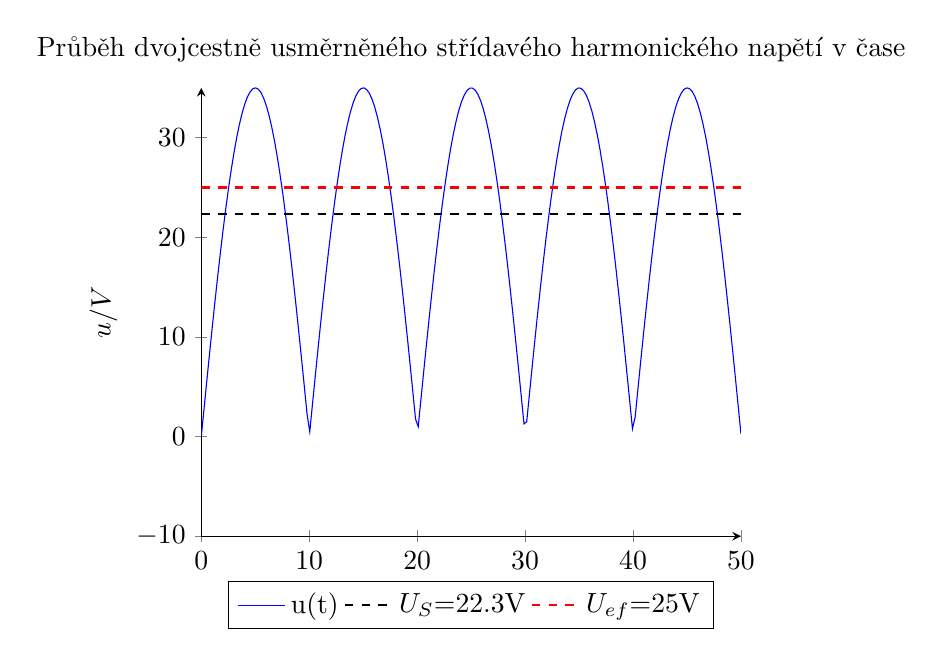
\begin{tikzpicture}
\label{grf:u_fullbridge_rectified}
\begin{axis}[
    title = {Průběh dvojcestně usměrněného střídavého harmonického napětí v čase},
    axis lines = left,
    ymin = -10,
    xlabel = \(t/ms\),
    ylabel = {\(u/V\)},
    legend style={at={(0.5,-0.1)}, anchor=north,legend columns=-1},
]

%Sinusovka
\addplot [
	domain=0:50,
	samples=200,
	color=blue,
]
{abs(35*sin(deg(2*3.14*50*x/1000)))};
\addlegendentry{u(t)}

%mean 
\addplot [
	domain=0:50,
	samples=200,
	color=black,
	thick,
	dashed,
]
{22.3};
\addlegendentry{$U_S$=22.3V}

%effective 
\addplot [
	domain=0:50,
	samples=200,
	color=red,
	thick,
	dashed,
]
{25};
\addlegendentry{$U_{ef}$=25V}

\end{axis}
\end{tikzpicture}
\end{center}

\subsection{Měřící soustavy elektrických analogových přístrojů a měření osciloskopem}

\paragraph{}
Analogové měřící přístroje měří základní elektrické veličiny (proud, napětí, odpor, činný výkon). Tyto přístroje jsou většinou konstruovány tak, že měří na principu vychýlení ručičky ciferníku působením magnetických silových polí. Tyto pole jsou většinou generovány přímo procházejícím proudem, nebo proudem, které v přístroji vytvoří měřené napětí. Pokud se jedná o stejnosměrný měřící přístroj, nesmí se zanedbat polarita. Analogové měřící přístroje mají většinou vnitřní odpor, který oproti digitálním měřícím přístrojům nemůžeme zanedbat.

\subsubsection{Třída přesnosti}
\paragraph{}
Třída přesnosti je parametr, který udává maximální chybu analogových přístrojů. Třída přesnosti se vyjadřuje v procentech a má označení $T_P$.
Pro určení mezní absolutní chyby platí následující vztah:

\begin{equation}
\label{eqn:mezní_absolutní_chyba}
\delta (U) = \frac{T_P}{100} \cdot U_R
\end{equation}

kde $U_R$ je zvolený rozsah voltmetru
\paragraph{}
Tato chyba je na celém zvoleném rozsahu stejná. Pokud chceme vypočítat relativní chybu, což je v procentech vyjádřený poměr absolutní chyby a naměřené hodnoty napětí, m;žeme použít následující vztah.

\begin{equation}
\label{eqn:relativní_chyba}
\delta _r (U) = \frac{\delta (U)}{U_{Měř}}\cdot 100%
\end{equation}
\paragraph{}
Z tohoto plyne, že chyba měření je výrazně nižší při měření ke konci stupnice. Proto se většinou snažíme docílit toho, aby se naměřená hodnota pohybovala v horní třetině rozsahu.

\subsubsection{Měřící přístroje s jedním rozsahem}
\paragraph{}
U tohoto typu měřících přístrojů ukazuje ručička na stupnici přímo hodnotu měřené veličiny. Tyto stupnice mohou být lineární, logaritmické či jinak nelineární, a také mohou mít potlačenou nulu, nebo prodlouženou stupnici. Pokud má přístroj prodlouženou stupnici, tak od místa označeným tečkou jsou hodnoty orientační - neodpovídají $T_p$ přístroje.

\subsubsection{Měřící přístroje s více rozsahy}
\paragraph{}
Tyto měřící přístroje mají jednu stupnici, ale více možných rozsahů. Ručička tudíž neudává přímo hodnotu měřené veličiny. Pro to, abychom získali skutečnou hodnotu měřené veličiny můžeme využít následující vztah. V tomto vztahu pro demonstraci použiji napětí.

\begin{equation}
\label{eqn:skutečná_naměřená_hodnota}
U=k\cdot \alpha ; \quad \quad \quad k = \frac{U_R}{\alpha _{max}}
\end{equation}
\paragraph{}
kde $\alpha$ je naměřený počet dílků stupnice, $\alpha _{max}$ je maximální počet dílků na stupnici a $U_R$ je zvolený rozsah napětí. Obdobně se počítájí hodnoty libovoné měřené veličiny.

\subsubsection{Měřící soustavy}
\paragraph{}
Analogové měřící přístroje mají různě principy měření. Na základě toho, co potřebujeme měřit je tedy nutné si vybrat příslušný typ měřícího přístroje.

\subsubsection{Přístroje magnetoelektrické}
\paragraph{}
Výchylka ručičky těchto přístrojů je přímo úměřná střední hodnotě měřené veličiny. Tyto přístroje reagují pouze na stejnosměřné proudy, a proto je nutné dbát na polaritu, Připojíme-li tento měřící přístroj na střídavý proud nízké frekvence, ručička se bude snažit sledovat změnu polarity proudu. Pokud zvýšíme dostatečně frekvenci, ručička již stíhat nebude a ustálí se na nule. Pokud se takto stane, a měřená veličina je dostatečně vysoká, může dojít ke zničení měřícího přístroje, nebo k ohrožení obsluhy tohot přístroje.

\subsubsection{Přístroje magnetoelektrické s usměrňovačem}
\paragraph{}
Tato soustava má velmi podobnou konstrukci jako mají přístroje magnetoelektrické, akorát mají předřazený usměrňovač, což jim umožňuje měřit i střídavé veličiny. Výchylka ručičky tohoto přístroje je [měrná střední hodnotě usměřněného průběhu měřené veličiny. Nevýhodou tohoto měřícího přístroje je to, že nemá lineární propustnost, což znamená že při jiných parametrech vstupního signálu, než na který byl konstruován, změřené hodnoty nemusí vypovídat skutečné hodnoty. Většina techto přístrojů je konstruována pro harmonický průběh při frekvenci 50Hz. Stupnice těchto přístrojů bývá cejchována v efektivních hodnotách, tudíž tato soustava měří efektivní hodnotu daného průběhu. Tudíž pokud chceme zjistit střední hodnotu průběhu, musíme měřenou hodnotu vydělit činitelem tvaru.

\subsubsection{Přístroje ferromagnetické (elektromagnetické)}
\paragraph{}
U těchto přístrojů je výchylka ručičky přímo [měrná efektivní hodnotě měřené veličiny, a stejně tak je i cejchována stupnice. Elektromagnetické přístroje jsou na výrobu nejjednodušší, ale jsou méňě citlivé a mohou zanechávat zkreslenější signál kvůli přechodným dějům než například přístroje magnetoelektrické.

\subsubsection{Osciloskop jako univerzální měřící přístroj}
\paragraph{}
Osciloskop je univerzální měřící přístroj, který na svém displeji ukazuje časové průběhy signálů, které jsou přivedeny na jeho kanály. Osciloskopy se dělí na digitální a analogové, dvoukanálové a vícekanálove. V této úloze využijeme digitální dvoukanálový osciloskop. Nastavení tohoto osciloskopu je oproti analogovému jednoduché, jelikož digitální osciloskopy bývají vybaveny tlačítkem autoscale.

\section{Princip metody měření}
\paragraph{}
Pro měření této úlohy jsme měli k dispozici přípravek, jehož zapojení je zobrazeno níže, dva uzly o 5-ti možných připojených zařízeních, digitální osciloskop a 3 analogové měřící přístroje (magnetoelektrický, magnetoelektrický s usměrnovačem a ferromagnetický).

\begin{center}
\begin{figure}[H]
\centering
\includegraphics[width=0.8\textwidth]{schema}
\caption{Schéma uspořádání prvku}
\label{img:schema}
\end{figure}
\end{center}

\paragraph{}
Z tohoto přípravku jsme během měření využili napětí 25V (mezi svorkami 30V a 5V), které jsme nejprve připojili na všechny měřící přístroje, až na magnetoelektricý. Dále jsme jeden přívodní vodič přípojili přes jednocestný usměrňovač realizovaný jednou diodou na všechny měřící přístroje. Nakonec jsme připojili všechny měřící přístroje na dvojcestný usměrňovač realizovaný Gretzovým můstkem napájeným transformátorem. Osciloskop jsme připojovali přes dělič 1:10.

\section{Naměřené hodnoty}

\begin{table}[H]
\resizebox{\columnwidth}{!}{%
\begin{tabular}{|lcc|ccc|ccc|ccc|}
\hline
\multicolumn{1}{|c|}{\begin{tabular}[c]{@{}c@{}}Jmenovitá hodnota\\ napětí na výstupu\\ transformátoru\\ 25V\end{tabular}} & \multicolumn{2}{c|}{\begin{tabular}[c]{@{}c@{}}Orientační měření \\ osciloskopem\end{tabular}}                                 & \multicolumn{3}{c|}{\begin{tabular}[c]{@{}c@{}}V1\\ \\ Magnetoelektrický voltmetr\\ TP 0.5\%\end{tabular}}                                                                                                                          & \multicolumn{3}{c|}{\begin{tabular}[c]{@{}c@{}}V2\\ \\ Magnetoelektrický voltmetr\\ s usměrňovačem\\ TP 0.5\%\end{tabular}}                                                                                                         & \multicolumn{3}{c|}{\begin{tabular}[c]{@{}c@{}}V3\\ \\ Ferromagtenický voltmetr\\ TP 0.5\%\end{tabular}}                                                                                                                            \\ \hline
\multicolumn{3}{|l|}{}                                                                                                                                                                                                                                      & \multicolumn{3}{c|}{$U_s$}                                                                                                                                                                                                             & \multicolumn{3}{c|}{$U_{ef}$}                                                                                                                                                                                                            & \multicolumn{3}{c|}{$U_{ef}$}                                                                                                                                                                                                            \\ \hline
\multicolumn{1}{|l|}{Měřený průběh}                                                                                        & \multicolumn{1}{c|}{\begin{tabular}[c]{@{}c@{}}u\\ {[}V{]}\end{tabular}} & \begin{tabular}[c]{@{}c@{}}u\\ {[}V{]}\end{tabular} & \multicolumn{1}{c|}{\begin{tabular}[c]{@{}c@{}}$\alpha$ \\ {[}dílek{]}\end{tabular}} & \multicolumn{1}{c|}{\begin{tabular}[c]{@{}c@{}}k\\ {[}V/dílek{]}\end{tabular}} & \begin{tabular}[c]{@{}c@{}}Umer = $\alpha$*k\\ {[}V{]}\end{tabular} & \multicolumn{1}{c|}{\begin{tabular}[c]{@{}c@{}}$\alpha$\\ {[}dílek{]}\end{tabular}} & \multicolumn{1}{c|}{\begin{tabular}[c]{@{}c@{}}k\\ {[}V/dílek{]}\end{tabular}} & \begin{tabular}[c]{@{}c@{}}Umer = $\alpha$*k\\ {[}V{]}\end{tabular} & \multicolumn{1}{c|}{\begin{tabular}[c]{@{}c@{}}$\alpha$\\ {[}dílek{]}\end{tabular}} & \multicolumn{1}{c|}{\begin{tabular}[c]{@{}c@{}}k\\ {[}V/dílek{]}\end{tabular}} & \begin{tabular}[c]{@{}c@{}}Umer = $\alpha$*k\\ {[}V{]}\end{tabular} \\ \hline
\multicolumn{1}{|l|}{\begin{tabular}[c]{@{}l@{}}Harmonický \\ neusměřněný\end{tabular}}                                    & \multicolumn{1}{c|}{64.3}                                                & 32.15                                               & \multicolumn{1}{c|}{-}                                                           & \multicolumn{1}{c|}{-}                                                         & -                                                               & \multicolumn{1}{c|}{49}                                                          & \multicolumn{1}{c|}{60/120}                                                    & 24.5                                                            & \multicolumn{1}{c|}{117}                                                         & \multicolumn{1}{c|}{26/130}                                                    & 23.4                                                            \\ \hline
\multicolumn{1}{|l|}{\begin{tabular}[c]{@{}l@{}}Jednocestně \\ usměrněný\end{tabular}}                                     & \multicolumn{1}{c|}{31.8}                                                & 31.1                                                & \multicolumn{1}{c|}{53}                                                          & \multicolumn{1}{c|}{24/120}                                                    & 10.6                                                            & \multicolumn{1}{c|}{62}                                                          & \multicolumn{1}{c|}{24/120}                                                    & 12.4                                                            & \multicolumn{1}{c|}{82.5}                                                        & \multicolumn{1}{c|}{26/130}                                                    & 16.5                                                            \\ \hline
\multicolumn{1}{|l|}{\begin{tabular}[c]{@{}l@{}}Dvoucestně \\ usměrněný\end{tabular}}                                      & \multicolumn{1}{c|}{31.0}                                                & 30.5                                                & \multicolumn{1}{c|}{105}                                                         & \multicolumn{1}{c|}{24/120}                                                    & 21                                                              & \multicolumn{1}{c|}{114}                                                         & \multicolumn{1}{c|}{24/120}                                                    & 22.8                                                            & \multicolumn{1}{c|}{113}                                                         & \multicolumn{1}{c|}{26/130}                                                    & 22.6                                                            \\ \hline
\end{tabular}%
}
\caption{Tabulka naměřených a vypočtených hodnot}
\label{tab:namerene_hodnoty}
\end{table}

\section{Zpracování hodnot}
\subsection{Harmonický neusměrněný průběh}

\begin{table}[H]
\centering
\resizebox{\columnwidth}{!}{%
\begin{tabular}{|c|c|c|c|c|c|c|c|c|}
\hline
\textbf{Měřidlo} &
  \begin{tabular}[c]{@{}c@{}}$U_{mer}$\\ {[}V{]}\end{tabular} &
  \begin{tabular}[c]{@{}c@{}}$\delta (U_{mer})$\\ {[}V{]}\end{tabular} &
  \begin{tabular}[c]{@{}c@{}}$U_{ef}$\\ {[}V{]}\end{tabular} &
  \begin{tabular}[c]{@{}c@{}}$U_s$\\ {[}V{]}\end{tabular} &
  \begin{tabular}[c]{@{}c@{}}$U_M$\\ {[}V{]}\end{tabular} &
  \begin{tabular}[c]{@{}c@{}}$\delta (U_M)$\\ {[}V{]}\end{tabular} &
  \begin{tabular}[c]{@{}c@{}}$\delta _r (U_M)$\\ {[}V{]}\end{tabular} &
  pozn. \\ \hline
\begin{tabular}[c]{@{}c@{}}Magnetoelektrický\\ Voltmetr\end{tabular} &
  - &
  - &
  - &
  - &
  - &
  - &
  - &
  \begin{tabular}[c]{@{}c@{}}Rozsah: -V\\ TP: 0.5\%\end{tabular} \\ \hline
\begin{tabular}[c]{@{}c@{}}Magnetoelektrický voltmetr\\ s usměrňovačem\end{tabular} &
  24.5 &
  0.9 &
  24.5 &
  0 &
  34.6 &
  1.3 &
  3.8 &
  \begin{tabular}[c]{@{}c@{}}Rozsah: 60V\\ TP: 1.5\%\end{tabular} \\ \hline
\begin{tabular}[c]{@{}c@{}}Elektromagnetický\\ (ferromagnetický) voltmetr\end{tabular} &
  23.4 &
  0.13 &
  23.4 &
  0 &
  33.1 &
  0.18 &
  0.5 &
  \begin{tabular}[c]{@{}c@{}}Rozsah: 26V\\ TP: 0.5\%\end{tabular} \\ \hline
\end{tabular}%
}
\caption{Průběh napětí: harmonický}
\label{tab:harmonicke_vypocty}
\end{table}

\subsubsection{Ukázka výpočtů pro magnetoelektrický voltmetr s usměrňovačem}
Mezní absolutní chyba
\begin{equation}
\label{eqn:vypocet_harm_meznichyba}
\delta (U) = \frac{T_p}{100}\cdot U_R = \frac{1.5}{100}\cdot 60=0.9V
\end{equation}

Amplituda vstupního signálu
\begin{equation}
\label{eqn:vypocet_harm_amplituda}
U_M = U_{ef} \cdot \sqrt{2} = 24.5 \cdot \sqrt{2} = 34.6V
\end{equation}

Absolutní chyba měření amplitudy
\begin{equation}
\label{eqn:vypocet_harm_abschyba_amp}
\delta (U_M) = \delta (U_{mer}) \cdot \sqrt{2} = 0.9 \cdot \sqrt{2} = 1.3V
\end{equation}

Relativní chyba měření amplitudy
\begin{equation}
\label{eqn:vypocet_harm_relchyba_amp}
\delta _r (U_M) = \frac{\delta (U_M)}{U_M}\cdot 100 = \frac{1.3}{34.6}\cdot 100 = 3.8 \%
\end{equation}

\subsection{Jednocestně usměrněný harmonický průběh}

\begin{table}[H]
\centering
\resizebox{\columnwidth}{!}{%
\begin{tabular}{|c|c|c|c|c|c|c|c|c|}
\hline
\textbf{Měřidlo} &
  \begin{tabular}[c]{@{}c@{}}$U_{mer}$\\ {[}V{]}\end{tabular} &
  \begin{tabular}[c]{@{}c@{}}$\delta (U_{mer})$\\ {[}V{]}\end{tabular} &
  \begin{tabular}[c]{@{}c@{}}$U_{ef}$\\ {[}V{]}\end{tabular} &
  \begin{tabular}[c]{@{}c@{}}$U_s$\\ {[}V{]}\end{tabular} &
  \begin{tabular}[c]{@{}c@{}}$U_M$\\ {[}V{]}\end{tabular} &
  \begin{tabular}[c]{@{}c@{}}$\delta (U_M)$\\ {[}V{]}\end{tabular} &
  \begin{tabular}[c]{@{}c@{}}$\delta _r (U_M)$\\ {[}V{]}\end{tabular} &
  pozn. \\ \hline
\begin{tabular}[c]{@{}c@{}}Magnetoelektrický\\ Voltmetr\end{tabular} &
  10.6 &
  0.12 &
  - &
  10.6 &
  33.3 &
  0.4 &
  1.2 &
  \begin{tabular}[c]{@{}c@{}}Rozsah: 24V\\ TP: 0.5\%\end{tabular} \\ \hline
\begin{tabular}[c]{@{}c@{}}Magnetoelektrický voltmetr\\ s usměrňovačem\end{tabular} &
  12.4 &
  0.4 &
  17.5 &
  - &
  35.1 &
  1.13 &
  3.2 &
  \begin{tabular}[c]{@{}c@{}}Rozsah: 24V\\ TP: 1.5\%\end{tabular} \\ \hline
\begin{tabular}[c]{@{}c@{}}Elektromagnetický\\ (ferromagnetický) voltmetr\end{tabular} &
  16.5 &
  0.13 &
  16.5 &
  - &
  33.0 &
  0.26 &
  0.8 &
  \begin{tabular}[c]{@{}c@{}}Rozsah: 26V\\ TP: 0.5\%\end{tabular} \\ \hline
\end{tabular}%
}
\caption{Průběh napětí: jednocestně usměrněný}
\label{tab:jednocestn_vypocty}
\end{table}

\subsubsection{Ukázka výpočtů pro magnetoelektrický voltmetr s usměřňovačem}
Mezní absolutní chyba
\begin{equation}
\label{eqn:vypocet_jedno_meznichyba}
\delta (U) = \frac{T_p}{100}\cdot U_R = \frac{1.5}{100}\cdot 24=0.4V
\end{equation}

Efektivni hodnota napětí
\begin{equation}
\label{eqn:vypocet_jedno_eff}
U_{ef} = U_{mer} \cdot\sqrt{2} = 12.4 \cdot\sqrt{2} = 17.5V
\end{equation}

Amplituda vstupního signálu
\begin{equation}
\label{eqn:vypocet_jedno_amplituda}
U_M = U_{mer} \cdot 2\sqrt{2} = 12.4 \cdot 2\sqrt{2} = 35.1V
\end{equation}

Absolutní chyba měření amplitudy
\begin{equation}
\label{eqn:vypocet_jedno_abschyba_amp}
\delta (U_M) = \delta (U_{mer}) \cdot 2\sqrt{2} = 0.4 \cdot 2\sqrt{2} = 1.13V
\end{equation}

Relativní chyba měření amplitudy
\begin{equation}
\label{eqn:vypocet_jedno_relchyba_amp}
\delta _r (U_M) = \frac{\delta (U_M)}{U_M}\cdot 100 = \frac{1.13}{35.1}\cdot 100 = 3.8 \%
\end{equation}

\subsection{Dvojcestně usměrněný harmonický průběh}

\begin{table}[H]
\centering
\resizebox{\columnwidth}{!}{%
\begin{tabular}{|c|c|c|c|c|c|c|c|c|}
\hline
\textbf{Měřidlo} &
  \begin{tabular}[c]{@{}c@{}}$U_{mer}$\\ {[}V{]}\end{tabular} &
  \begin{tabular}[c]{@{}c@{}}$\delta (U_{mer})$\\ {[}V{]}\end{tabular} &
  \begin{tabular}[c]{@{}c@{}}$U_{ef}$\\ {[}V{]}\end{tabular} &
  \begin{tabular}[c]{@{}c@{}}$U_s$\\ {[}V{]}\end{tabular} &
  \begin{tabular}[c]{@{}c@{}}$U_M$\\ {[}V{]}\end{tabular} &
  \begin{tabular}[c]{@{}c@{}}$\delta (U_M)$\\ {[}V{]}\end{tabular} &
  \begin{tabular}[c]{@{}c@{}}$\delta _r (U_M)$\\ {[}V{]}\end{tabular} &
  pozn. \\ \hline
\begin{tabular}[c]{@{}c@{}}Magnetoelektrický\\ Voltmetr\end{tabular} &
  21 &
  0.12 &
  - &
  21 &
  33.0 &
  0.19 &
  0.6 &
  \begin{tabular}[c]{@{}c@{}}Rozsah: 24V\\ TP: 0.5\%\end{tabular} \\ \hline
\begin{tabular}[c]{@{}c@{}}Magnetoelektrický voltmetr\\ s usměrňovačem\end{tabular} &
  22.8 &
  0.4 &
  22.8 &
  - &
  32.2 &
  0.6 &
  1.8 &
  \begin{tabular}[c]{@{}c@{}}Rozsah: 24V\\ TP: 1.5\%\end{tabular} \\ \hline
\begin{tabular}[c]{@{}c@{}}Elektromagnetický\\ (ferromagnetický) voltmetr\end{tabular} &
  22.6 &
  0.13 &
  22.6 &
  - &
  32.0 &
  0.18 &
  0.6 &
  \begin{tabular}[c]{@{}c@{}}Rozsah: 26V\\ TP: 0.5\%\end{tabular} \\ \hline
\end{tabular}%
}
\caption{Průběh napětí: dvojcestně usměrněný}
\label{tab:dvojcest_vypocty}
\end{table}

\subsubsection{Ukázka výpočtů pro elektromagnetický (ferromagnetický) voltmetr}
Mezní absolutní chyba
\begin{equation}
\label{eqn:vypocet_jedno_meznichyba}
\delta (U) = \frac{T_p}{100}\cdot U_R = \frac{0.5}{100}\cdot 26=0.13V
\end{equation}

Amplituda vstupního signálu
\begin{equation}
\label{eqn:vypocet_jedno_amplituda}
U_M = U_{ef} \cdot \sqrt{2} = 22.6 \cdot \sqrt{2} = 32.0V
\end{equation}

Absolutní chyba měření amplitudy
\begin{equation}
\label{eqn:vypocet_jedno_abschyba_amp}
\delta (U_M) = \delta (U_{mer}) \cdot \sqrt{2} = 0.13 \cdot\sqrt{2} = 0.18V
\end{equation}

Relativní chyba měření amplitudy
\begin{equation}
\label{eqn:vypocet_jedno_relchyba_amp}
\delta _r (U_M) = \frac{\delta (U_M)}{U_M}\cdot 100 = \frac{0.18}{32.0}\cdot 100 = 0.6 \%
\end{equation}

\subsection{Shrnutí vypočtených hodnot}

\begin{table}[H]
\centering
\resizebox{\columnwidth}{!}{%
\begin{tabular}{|c|c|ccc|ccc|ccc|}
\hline
\begin{tabular}[c]{@{}c@{}}Jmenovitý výstup\\ transformátoru\end{tabular} &
  \begin{tabular}[c]{@{}c@{}}Osciloskop\\ orientačně\end{tabular} &
  \multicolumn{3}{c|}{\begin{tabular}[c]{@{}c@{}}Magnetoelektrický voltmetr\\ TP 0.5\%\end{tabular}} &
  \multicolumn{3}{c|}{\begin{tabular}[c]{@{}c@{}}Magnetoelektrický voltmetr\\ s usměrňovačem TP 1.5\%\end{tabular}} &
  \multicolumn{3}{c|}{\begin{tabular}[c]{@{}c@{}}Elektromagnetický voltmetr\\ (ferromagnetický) TP 0.5\%\end{tabular}} \\ \hline
\textbf{25V} &
  $U_M$ &
  \multicolumn{1}{c|}{$U_M$} &
  \multicolumn{1}{c|}{$\delta (U_M)$} &
  $\delta (U_M)$ &
  \multicolumn{1}{c|}{$U_M$} &
  \multicolumn{1}{c|}{$\delta (U_M)$} &
  $\delta (U_M)$ &
  \multicolumn{1}{c|}{$U_M$} &
  \multicolumn{1}{c|}{$\delta (U_M)$} &
  $\delta (U_M)$ \\ \hline
Měřený průběh &
  {[}V{]} &
  \multicolumn{1}{c|}{{[}V{]}} &
  \multicolumn{1}{c|}{{[}V{]}} &
  {[}\%{]} &
  \multicolumn{1}{c|}{{[}V{]}} &
  \multicolumn{1}{c|}{{[}V{]}} &
  {[}\%{]} &
  \multicolumn{1}{c|}{{[}V{]}} &
  \multicolumn{1}{c|}{{[}V{]}} &
  {[}\%{]} \\ \hline
\begin{tabular}[c]{@{}c@{}}Harmonické\\ (neusměrněné)\end{tabular} &
  32.15 &
  \multicolumn{1}{c|}{-} &
  \multicolumn{1}{c|}{-} &
  - &
  \multicolumn{1}{c|}{34.6} &
  \multicolumn{1}{c|}{1.3} &
  3.8 &
  \multicolumn{1}{c|}{33.1} &
  \multicolumn{1}{c|}{0.18} &
  0.5 \\ \hline
\begin{tabular}[c]{@{}c@{}}Jednocestně\\ usměrněné\end{tabular} &
  31.1 &
  \multicolumn{1}{c|}{33.3} &
  \multicolumn{1}{c|}{0.4} &
  1.2 &
  \multicolumn{1}{c|}{35.1} &
  \multicolumn{1}{c|}{1.13} &
  3.2 &
  \multicolumn{1}{c|}{33.0} &
  \multicolumn{1}{c|}{0.26} &
  0.8 \\ \hline
\begin{tabular}[c]{@{}c@{}}Dvoucestně\\ usměrněné\end{tabular} &
  30.5 &
  \multicolumn{1}{c|}{33.0} &
  \multicolumn{1}{c|}{0.19} &
  0.6 &
  \multicolumn{1}{c|}{32.2} &
  \multicolumn{1}{c|}{0.6} &
  1.8 &
  \multicolumn{1}{c|}{32.0} &
  \multicolumn{1}{c|}{0.18} &
  0.6 \\ \hline
\end{tabular}%
}
\caption{Přehledná tabulka velikostí amplitud a jejich absolutních a relativních chyb}
\label{tab:vypocy_shrnuti}
\end{table}

\section{Použité přístroje}
\begin{table}[H]
\centering
\resizebox{\columnwidth}{!}{%
\begin{tabular}{|l|l|l|l|}
\hline
\multicolumn{1}{|c|}{\begin{tabular}[c]{@{}c@{}}Označení\\ ve schématu\end{tabular}} &
  \multicolumn{1}{c|}{Název} &
  \multicolumn{1}{c|}{\begin{tabular}[c]{@{}c@{}}Identifikace\\ (výrobní číslo)\end{tabular}} &
  \multicolumn{1}{c|}{\begin{tabular}[c]{@{}c@{}}Doplňkové\\ údaje\end{tabular}} \\ \hline
V1         & DKP661               & 1000004877 & TP 0,5\% DC, ELP2, horizont. poloha \\ \hline
V2         & DKP850               & 1060005264 & TP 1,5\% AC, ELP2, horizont. poloha \\ \hline
V3         & DKP536               & 1000004433 & TP 0,5\% AC, ELP2, horizont. poloha \\ \hline
Osciloskop & Keysight EDUX 1002 A & CN57350373 & 50 MHz, 16 GSa/s                    \\ \hline
\end{tabular}%
}
\caption{Tabulka použitých přístrojů}
\end{table}

\section{Závěr}
\paragraph{}
Z naměřených hodnot amplitud napětí (viz. sekce Shrnutí vypočtených hodnot) lze vypozorovat na základě porovnání vypočtených amplitud ve všech měřených průbězích na jednotlivých voltmetrech, že nejméně kolísala hodnota napětí u elektromagnetického voltmetru. Pokud bychom se omezili pouze na usměrněné průběhy, lepší výsledky by měl magnetoelektrický voltmetr bez usměrňovače. Vyšší odchylky magnetoelektrického voltmetru s usměrňovačem mohly být zapříčiňeny úbytkem napětí na diodách. 

\paragraph{}
Hodnoty měřené osciloskopem mají výrazně vyšší odchylku, než hodnoty měřené analogovými přístroji. Tato chyba mohla být hlavně způsobena nepřesnou děličkou 1:10, která nebyla proměřována. Další chyba mohla být způsobena vlivem ostatních měřících přístrojů.

\end{document}

